\documentclass[11pt]{article}
\usepackage{mathpazo}
\usepackage{fullpage}
\usepackage{amsmath}
\usepackage{amssymb}
\usepackage{epsfig}
\usepackage{graphicx}
\usepackage{color}
\usepackage{wasysym}

%%% TEMPLATE PREAMBLE STARTS HERE
\def\classname{Foundations of Cryptography}
\def\classnumber{CS579/CpE579}
\def\classterm{Spring 2011}
\def\lecturenumeral{10}
\def\scribedate{6 April 2011}
\def\pageheader{\classnumber: Lecture \lecturenumeral}
\def\instructor{Antonio R.\@ Nicolosi}
\def\scribe{Vincent Lin}

\newcommand{\mathsym}[1]{{}}

\def\therefore{
\leavevmode
\lower0.1ex\hbox{$\bullet$}
\kern-0.2em\raise0.7ex\hbox{$\bullet$}
\kern-0.2em\lower0.2ex\hbox{$\bullet$}
\thinspace}

\renewcommand\thepage{L\lecturenumeral-\arabic{page}}

\newcommand{\blank}{\underline{\hbox to2in{\hss}}}

\newtheorem{lemma}{Lemma}

\begin{document}


\medskip

\begin{center}
{\LARGE \classname}

\smallskip

\noindent
{\small
\classnumber---\classterm}
\end{center}

\medskip

\noindent
Instructor: \instructor \hfill Scribe: \scribe

\medskip

\hrule

\medskip
\noindent
Lecture \lecturenumeral
  \hfill
\scribedate
%%% TEMPLATE PREAMBLE ENDS HERE

\section{Reverse Homework Review}
\subsection{Encryption and Message Authentication Codes (MACs)}
In Lab 1 we have a system where we apply AES during CBC to encrypt the message,
and then take the result and hash it with HMAC-SHA1:\\*
$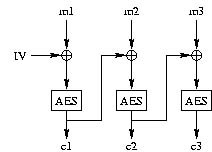
\includegraphics[scale=0.65]{cbc.jpg}$\\*
($c_0c_1c_2\ldots$ is then hashed with HMAC-SHA1 and the result is appended to
the end of the encrypted file.)\\*\\*
But what if we do encryption/MAC in a different order?
\begin{itemize}
  \item Encrypt then MAC (the method described above)\\*
  \indent This is what is used in Lab 1, and it always works while satisfying
  our definition of security.
  \item MAC then Encrypt\\*
  \indent This works most of the time, but there exists an issue with it that
  will be discussed later.
  \item Encrypt $\mid \mid$ MAC\\*
  \indent (Here we append the MAC of the original message to
  the end of the encryption of that same message.)  This method is broken because it does not satisfy our definition of security.
\end{itemize}
\subsection{Definition of Security}
  Building upon our original definition of security, we can make the game easier
  for the attacker by giving access to an encryption oracle that takes an input
  $m^i$ and returns the ciphertext created by encrypting $m^i$ with the selected
  encryption key:\\*
  $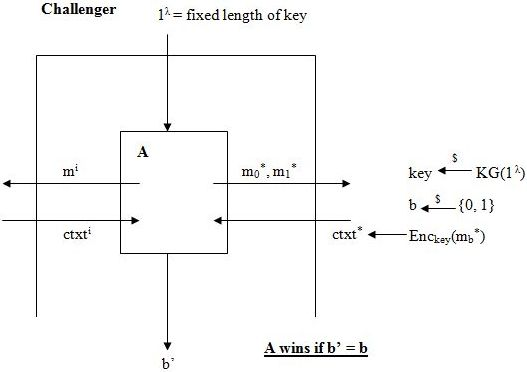
\includegraphics[scale=0.81]{security.jpg}$\\*
  More formally, $\forall$ efficient attackers A,\\*
  \indent $\exists$ $\gamma$ \makebox[0.25in][r]{s.t.} Pr[ b = b' $\mid$ k
  $\leftarrow$ KG($1^{\lambda}$), b $\leftarrow \{$0, 1$\}$, b' $\leftarrow
  A^{Enc(k,\cdot)}$, Enc(k, select(b,$\cdot$,$\cdot$))] $\leq \frac{1}{2}$ +
  $\gamma$\\* 
  (*It should be noted that this updated game will never work with a
  deterministic encryption scheme.  In general, a secure encryption scheme can
  never be deterministic.)
  
\subsection{Encrypt $\mid \mid$ MAC}
  Now consider Encrypting using AES-CBC and hashing with HMAC-SHA1:\\*
  $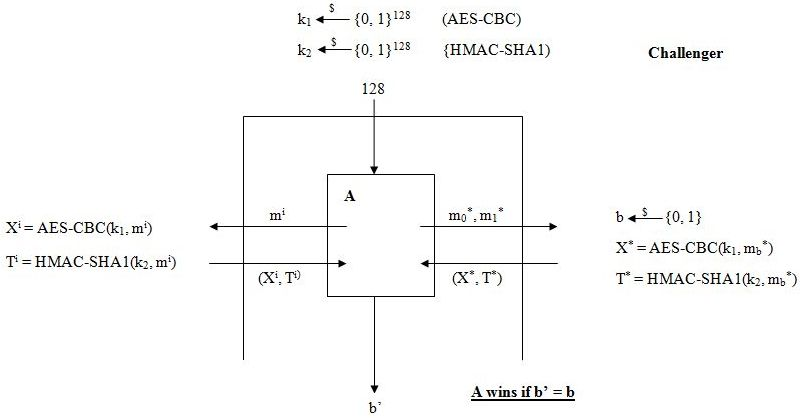
\includegraphics[scale=0.75]{security2.jpg}$\\*
  Since HMAC-SHA1 is deterministic by construction, the second portion of the
  ciphertext is generated deterministically and the scheme is broken.  An
  attacker can just compare T's.\\*\\*
  MACs are used for data integrity and authentication.  If you want secrecy, you
  need encryption, and if you want to combine them, you should encrypt the
  message first and then use the ciphertext for appended MACs instead of using
  the plaintext.
  
\subsection{MAC then Encrypt}
  The one caveat for MAC then Encrypt has to do with message length.  If we do
  not specify that $\mid m^*_0 \mid = \mid m^*_1 \mid$ then the scheme has a
  problem.  Encryption does not guarantee the protection of the size of the
  file.  If one message is 1 byte and the other is 1 terrabyte, the ciphertext
  sizes could be very different in size.  This does not matter for our library
  because HMAC-SHA1 takes a message of any length up to $2^{64}$ bytes and
  hashes it to a 20-byte output.  This guarantees that all messages being encrypted
  will be the same length, but this may not be the case with other MAC
  protocols.\\*\\*
  There is no requirement that forces MACs to always generate the same sized
  output from any input, and it is also okay for messages of the same length to
  have MACs of different length.\\*
  e.g. compression - Some files do not compress as well as others (think text
  files vs images) so 2 files of the same length originally might compress to
  different lengths.  So compressing and then MACing might cause the MACs
  generated to have different lengths before you encrypt the files, and result
  in ciphertexts of very different lengths.

\section{Modulo Group Theory}
\subsection{Review}
($\mathbb{Z}_{n}$, +) always works as an additive group:

\begin{itemize}
\item $\mathbb{Z}_{n}$ is closed under the group operation (addition):\\*
$\forall$ a, b $\in$ $\mathbb{Z}_{n}$, (a + b) $\in$
$\mathbb{Z}_{n}$.

\item The identity element, e, exists:\\* 
$\forall$ a $\in$ $\mathbb{Z}_{n}$, a = a + 0 = 0 + a = a.

\item ($\mathbb{Z}_{n}$, +) has the associative property:\\*
$\forall$ a, b, c $\in$ $\mathbb{Z}_{n}$, (a + b) + c = a + (b + c).

\item All elements of $\mathbb{Z}_{n}$ have an inverse:\\*
$\forall$ a $\in$ $\mathbb{Z}_{n}$, $\exists$ $a^{-1}$ \makebox[0.5in]{s.t.} e =
a + $a^{-1}$ = $a^{-1}$ + a = e
\end{itemize}

\noindent However this is not the case under multiplication.
For example, ($\mathbb{Z}_{26}$, $\cdot$) is closed, has an identity element
(1), and is associative, but not every element in ($\mathbb{Z}_{26}$, $\cdot$) 
has an inverse:\\*
\indent Inverses: $\forall$ a $\in$ $\mathbb{Z}_{26}$ $\exists$ $a^{-1}$
\makebox[0.5in]{s.t.} a $\cdot$ $a^{-1}$ = 1 mod 26 $\Longleftrightarrow$ gcd(a,
26) = 1\\*\\* \indent gcd(2, 26) = 2 $\ne$ 1 $\Longrightarrow$ 2 does not have an inverse in
($\mathbb{Z}_{26}$, $\cdot$) $\Longrightarrow$ ($\mathbb{Z}_{26}$, $\cdot$) is not a
group

\subsection{Compute Inverse Mod(a, n)}
This algorithm takes n and a, and returns the
inverse of a in $\mathbb{Z}_{n}$:\\*
\emph{\indent $x_{old}$ = n, $x_{curr}$ = a, $x_{new}$\\*
\indent $s_{old}$ = 1, $s_{curr}$ = 0, $s_{new}$\\*
\indent $t_{old}$ = 0, $t_{curr}$ = 1, $t_{new}$\\*\\*
\indent while $x_{curr}$ $>$ 0\\*
\indent \indent q = $\lfloor$$x_{old}$/$x_{curr}$$\rfloor$\\*
\indent \indent $x_{new}$ = $x_{old}$ - q*($x_{curr}$)\\*
\indent \indent $s_{new}$ = $s_{old}$ - q*($s_{curr}$)\\*
\indent \indent $t_{new}$ = $t_{old}$ - q*($t_{curr}$)\\*
\indent done\\*
\indent assert $x_{curr}$ == 1\\*
\indent return $s_{curr}$}\\*
(As mentioned in class, when only looking for the inverse of a, t is not used
in the algorithm, but it is necessary in order to prove that this algorithm
outputs the correct values.)

\subsection{$\mathbb{Z}^*_{n}$}
Now we continue with the issue from 1.1 where $\mathbb{Z}_{26}$ is not a group
because gcd(2, 26) = 2 $\neq$ 1.  In order to satisfy the Inverses axiom, all
elements of the set must be relatively prime to 26 (gcd(a, 26) = 1).  Now
consider a set $\mathbb{Z}^*_{26}$ defined as follows:\\*\\*
\indent $\mathbb{Z}^*_{26}$ := \{a $\in$ $\mathbb{Z}_{26}$
\makebox[0.25in][r]{s.t.} gcd(a, 26) = 1\}\\*
(This is essentially all of the numbers in $\mathbb{Z}_{26}$ that are
relatively prime with 26.  Because they are relatively prime, they must
also have inverses)
\subsubsection{Is ($\mathbb{Z}^*_{26}$, $\cdot$) a group?}
\begin{itemize}
  \item \emph{Identity}: 1 is inherited from ($\mathbb{Z}_{26}$, $\cdot$) as the
  identity.
  \item \emph{Associativity}: this is inherited from ($\mathbb{Z}_{26}$, $\cdot$).
  \item \emph{Existence of Inverses}: Everything must have an inverse since we
  constructed $\mathbb{Z}^*_{26}$ specifically so that all elements would have
  an inverse.
  \item \emph{Closure}: This is the only non-trivial one, but since gcd(a mod n,
  n) = 1 \& gcd(b mod n, n = 1) $\Longrightarrow$ gcd(a $\cdot$ b mod n, n) = 1, we know
  that $\mathbb{Z}^*_{26}$ is closed under multiplication.
\end{itemize}
Yes ($\mathbb{Z}^*_{26}$, $\cdot$) is a group, and we can generalize this to
($\mathbb{Z}_{n}$, $\cdot$)
\subsubsection{What is the size of $\mathbb{Z}^*_{n}$?}
$\lvert$$\mathbb{Z}_{n}$$\rvert$ = n\\*
$\lvert$$\mathbb{Z}^*_{n}$$\rvert$ $<$ n $\rightarrow$
$\lvert$$\mathbb{Z}^*_{n}$$\rvert$ $<$ n - p - q + 1 if n is a composite number
where n = pq (p, q prime and p $\neq$ q):\\*
\indent n - p - q + 1 = pq - p - q + 1 = p(q - 1) - (q - 1) = (p - 1)(q - 1) =
$\lvert$$\mathbb{Z}^*_{p}$$\rvert \cdot \lvert$$\mathbb{Z}^*_{q}$$\rvert$\\*
$\lvert$$\mathbb{Z}^*_{p}$$\rvert$ = p - 1 if p is prime (everything in
$\mathbb{Z}_{n}$ is coprime to p, and we do not include 0)\\* \indent p prime
$\Longrightarrow$ gcd(a, p) = 1 $\forall$ a $\in$ $\mathbb{Z}_{p}$$\backslash$$\{$0$\}$

\subsection{Euler Totient Function}
The Euler Phi function, as it is also refered to, is used to more easily compute
the number of elements in $\mathbb{Z}^*_n$ ($\phi$(n) =
$\lvert$$\mathbb{Z}^*_{n}$$\rvert$).\\*\\*
We know that $\phi$(p) = $\lvert$$\mathbb{Z}^*_{p}$$\rvert$ = p - 1 (p
prime).\\*
This also gives us $\phi$(p$\cdot$q)= $\phi$(p)$\cdot$$\phi$(q) (p, q prime and
p $\neq$ q)\\*
For general n, $\phi$($p^{e_1}_1$$\cdot$\ldots$\cdot$$p^{e_r}_r$) =
$\phi$($p^{e_1}_1$)$\cdot$\ldots$\cdot\phi$($p^{e_r}_r$) = $p^{e_1-1}_1$($p_1$
- 1)$\cdot$\ldots$\cdot$$p^{e_r-1}_r$($p_r$ - r)\\*\\*
Knowing the factorization of n is essentially like knowing the order of
$\mathbb{Z}^*_{n}$

\subsection{Prime Numbers}
\subsubsection{Density of primes in $\mathbb{Z}$}
Specifically, in the range 0 to $2^k$, what is the total number of primes?\\*
The number of primes is roughly $\theta$($\frac{2^k}{k}$) $\Longrightarrow$ in
the range 0 to m, the number of primes is roughly
$\theta$($\frac{m}{log(m)}$)\\*\\* We can now use this to find the expected
number of iterations that it would take to select a random number from 0 to k and check if it is prime:\\*
Pr[prime] = $\frac{\frac{2^k}{k}}{2^k}$ = $\frac{1}{k}$ $\Longrightarrow$
E(prime) = $\frac{1}{\frac{1}{k}}$ = k

\subsubsection{Testing the primality of r}
\emph{for i $\leftarrow$ 1 to $\sqrt{r}$ do\\*
\indent if $\frac{r}{i}$ is an integer (r mod i == 0)\\*
\indent \indent no\\*
yes}\\*\\*
This is a very naive algorithm to simply test all possible values up to
$\sqrt{r}$ to see if r is a prime.  Say r = 512 bits (r $\approx$ $2^{512}$). 
The loop runs for $\sqrt{2^{512}}$ = $2^{256}$.  This is not polynomial time,
and the run time is O($2^\frac{k}{2}$).\\*\\*
Other tests:
\begin{itemize}
  \item \emph{Miller-Rabin}: O($k^2$) (Probabilistic polynomial time)\\*
  \indent Returns either 'yes it is composite' or 'I don't know'
  \item \emph{AKS (2002)}: O($k^11$)\\*
  \indent This test does go through all possible values, and is deterministic.
  It has been improved since its development to O($k^6$), however running
  Miller-Rabin multiple times is still generally preferred.
\end{itemize}

\subsection{Cyclic Groups}
\subsubsection{Fermat's Little Theorem}
For p prime,\\*\\*
$\forall$ a $\in$ $\mathbb{Z}^*_{p}$ \makebox[0.125in]{}$a^{p-1} \cong$ 1 mod p.

\subsubsection{Definition of a Cyclic Group}
A cyclic group is defined as a group where all elements can be represented as
powers of a single element, called a generator (sometimes denoted with g).\\*\\*
More formally, a group, G, is said to be cylic if $\exists$ a $\in$ G
s.t. G = $\{$1, a, $a^2$, ..., $a^{\phi(n)-1} \}$

\subsubsection{Examples of Cyclic Groups}
($\mathbb{Z}_{n}$, +) is always a cyclic group because you can simply take
1 and add 1 repeatedly to generate all elements of the set
$\mathbb{Z}_{n}$.\\*\\*
($\mathbb{Z}^*_7$, $\cdot$) is also a cyclic group:\\*
($\mathbb{Z}^*_7$, $\cdot$) = $\{$1,2,3,4,5,6$\}$\\*
Now lets try to find a generator, we will test 2.\\*
\indent $2^0$mod(7)$\cong$1, \indent $2^1$mod(7)$\cong$2, \indent
$2^2$mod(7)$\cong$4, \indent $2^3$mod(7)$\cong$1, $\XBox$\\* 
Now 3,\\*
\indent $3^0$mod(7)$\cong$1, \indent $3^1$mod(7)$\cong$3, \indent
$3^2$mod(7)$\cong$2, \indent $3^3$mod(7)$\cong$6,\\*
\indent $3^4$mod(7)$\cong$4,
\indent $3^5$mod(7)$\cong$5, \indent $3^6$mod(7)$\cong$1, $\checkmark$

\subsubsection{The Order of $\mathbb{Z}^*_n$ and g}
(As mentioned above, g is called a generator or a
primitive root).\\*
G = ($\mathbb{Z}^*_{p}$, $\cdot$) is a cyclic group $\Longleftrightarrow$ $\exists$ g
$\in$ $\mathbb{Z}^*_{p}$ \makebox[0.25in]{s.t.} $\mathbb{Z}^*_{p}$ = $\{$1,
g, $g^2$, $g^3$,\ldots$\}$\\*\\*
Since $\mathbb{Z}^*_{p}$ is finite while the powers of g
can go up infinitely, we know that the powers of g must wrap around at some
point (pidgeonhole principle).\\*
e.g $g^r$ mod p = 1 where r is called the order of the element g.  This is
denoted as ord(g) = r\\*
So from our 2 examples in the previous section, ord(2) in ($\mathbb{Z}^*_7$, $\cdot$)
is 3 and ord(3) is 6.\\*\\*
The order of G = ($\mathbb{Z}^*_p$, $\cdot$) is the order of its generator
$\Rightarrow$ the order of $\mathbb{Z}^*_p$ is p - 1.  This can also be denoted
as $\lvert$G$\rvert$ = p - 1\\*\\*
Going back to Fermat's Little Theorem, if an element is in
$\mathbb{Z}^*_p$ and p prime, its order is always p - 1 or a factor of p - 1.

\subsubsection{Lagrange's Theorem}
If H is a subgroup of G (H $<$ G) then
$\frac{\lvert H\rvert}{\lvert G\rvert}$ (the order of H divides the order of
G)\\*
e.g. H = $\{$1, 2, 4$\}$ $<$ ($\mathbb{Z}^*_7$, $\cdot$) = $\{$1, 2, 3, 4, 5, 6$\}$
= G\\*\\*
H is closed:
\begin{verbatim}
		  | 1 | 2 | 4 |
		----------------
		1 | 1 | 2 | 4 |
		----------------
		2 | 2 | 4 | 1 |
		----------------
		4 | 4 | 1 | 2 |		(the multiplication table for {1, 2, 4}
\end{verbatim}
1 is the identity element, and all elements have an inverse (1's inverse is
itself, and 2 and 4 are the inverses of one another).  Associativity is
inherited from G so H is a group itself as well as a subgroup of G.\\*
$\lvert$G$\rvert$ = $\lvert$$\mathbb{Z}^*_7$$\rvert$ = p - 1 = 6\\*
$\lvert$H$\rvert$ = $\lvert$$\{$1, 2, 4$\}$$\rvert$ = 3\\*
3$\mid$6 $\checkmark$\\*\\*
$<$a$>$ = $\{$a, $a^2$ mod p,\ldots,$a^r$ mod p,\ldots$\}$ ($<$a$>$ denotes
that a is a generator)\\*\\*
By closure, we get that: ($a^i$ mod p) $\cdot$ ($a^j$ mod p) = $a^{i+j}$ mod p\\*\\*
o = ord(a)$\mid$(p - 1)\\* p - 1 = o $\cdot$ c (for some constant c)\\*
$\Rightarrow$ $a^o$ mod p = 1 (by the definition of the order of an element)\\*
= $a^{o \cdot c}$ = $1^c$ = 1 mod p\\*
= $a^{p-1}$ = 1 mod p (but this does not include 0 since 0 $\notin$
$\mathbb{Z}^*_p$)\\*
= $a^p \cdot a^{-1}$ = 1 mod p (using the property gained from closure)\\*
$\Longrightarrow a^p \cdot a^{-1} \cdot$ a = (1 mod p) $\cdot$ a\\*
$\Longrightarrow a^p$ = a mod p\\*\\*
To generalize: $\forall$ a $\in$ $\mathbb{Z}_p$, \makebox[0.25in]{}$a^p \cong$
a mod p

\subsection{Discrete Logarithms}
We already know that 3 is a generator of $\mathbb{Z}^*_7$.\\*\\*
$<$3$>$ = $\{$1, 3, 2, 6, 4, 5$\}$\\*
\indent (1 = $3^0$ mod 7) \indent (3 = $3^1$ mod 7) \indent (2 = $3^2$ mod 7)\\*
\indent (6 = $3^3$ mod 7) \indent (4 = $3^4$ mod 7) \indent (5 = $3^5$ mod
7)\\*\\* Now consider the following function \emph{f(x)}:
$\mathbb{Z}_{p-1} \rightarrow \mathbb{Z}^*_p$\\*
e.g. $\mathbb{Z}_{6} \rightarrow \mathbb{Z}^*_7$\\*
\indent x $\mid \rightarrow$ $3^x$ mod 7\\*
\indent 0 $\rightarrow$ 1\\*
\indent 1 $\rightarrow$ 3\\*
\indent 2 $\rightarrow$ 2\\*
\indent 3 $\rightarrow$ 6\\*
\indent 4 $\rightarrow$ 4\\*
\indent 5 $\rightarrow$ 5\\*
\emph{f} is a bijection and raising a base to an exponent over a
modulus is called modular exponentiation.\\*\\*
The inverse function of f is:\\*
$\mathbb{Z}^*_p \rightarrow \mathbb{Z}_{p-1}$\\*
y $\mid \rightarrow$ \makebox[0.25in]{s.t.} $3^x$ = y mod 7\\*\\*
This function is called the Discrete Logarithm (Dlog.\\*
e.g \indent $Dlog_3$ 6  = 3 $\Longrightarrow$ $3^3$ mod 7 = 6 $\checkmark$

\subsubsection{Efficiency}
For large numbers, $g^x$ mod p, you don't want to compute $g^x$ and then
reduce:\\*
\indent e.g.\indent $\lvert$g$\rvert$ = 1024 bits ($2^{1024}$)\\*
\indent e.g.\indent $\lvert$x$\rvert$ = 160 bits ($2^{160}$)\\*
\indent e.g.\indent $\lvert$p$\rvert$ = 1024 bits ($2^{1024}$)\\*\\*
$g^x$ = $(2^{1024})^{2^{160}} \sim (2^{2^{10}})^{2^{160}} \sim 2^{2^{170}} \sim
2^{170}$ \indent (too many steps)\\*\\*
Possible solution:\\*
 Try \indent g \indent $g^2$ \indent $g^3$ \indent \ldots \indent $g^x$\\*
 and do (mod p) at each step so that you don't grow in size.  Unfortunately this
 doesn't work because there are too many steps to take (x steps).  In the above
 example, $\lvert$x$\rvert$ = 160 bits $\Longrightarrow \approx 2^{160}$ steps.
 $\Longrightarrow$ too many steps.
 
\subsubsection{Horner's Rules of Multiplication}
 x : 160-bits\\*
 $(x_{159} x_{158} \ldots x_1 x_0)_2$ = x (binary representation of x)\\*
 $\Longrightarrow$ x = $x_0 + x_12^1 + x_22^2 + \ldots + x_{159}2^{159}$\\*
 \indent = $\displaystyle\sum\limits_{i=0}^{159} x_i2^i$\\*\\*
 To compute modular computation:\\*
 \indent $g^x$ = $g^{x_0+x_12^1+\ldots+x_{159}2^{159}}$\\*
 \indent \indent = $g^{x_0} g^{2(x_1+\ldots+x_{159}2^{159})}$\\*
 \indent \indent = $g^{x_0} g^{(x_1+\ldots+x_{159}2^{159})2}$\\*\\*
 So now consider a recursive algorithm to calculate modular exponentiation
 called ModExp:\\*
 ModExp(g, p, x, k) (where k = log(x))\\*
 \indent O(k) \indent ModExp k - 1 bits\\*
 \indent O($k^2$) \indent squaring mod p\\*
 \indent O($k^2$) \indent multiplication mod p\\*\\*
 Square + Multiply algorithm gives us a O($k^3$) run time to calculate modular
 exponentiate, which is efficient.
 
\begin{thebibliography}{99}
\bibitem[1]{Lecture notes} Lecture Notes. 'CS579 Foundations of Cryptography'.
Antonio Nicolosi. April 6. 2011.
\bibitem[2]{Scribe notes} Scribe Notes. 'CS579 Foundations of Cryptography'. Joe
Geis. April 14. 2010.
\end{thebibliography}

\end{document}